% Chapter 5

\chapter{Evaluation} % Methodology

\label{Chapter5} % For referencing the chapter elsewhere, use \ref{Chapter5} 

In this chapter we present the results of the evaluation starting with the best result obtained from each model from different hyper-parameter testing.

The performance of each model is then discussed further in the sections that follow. 

\section{Results summary}

Within the context of a home audio decide, the cost of mistakenly suggesting a user wants to listen to music is higher than the cost of not suggesting at all. We therefore focus our results on the predictions where a 'play' event was predicted by the model and examine both the precision and recall scores for both the hidden periods for existing users as well as new users.

All models required a number of runs to try and determine the best hyper-parameters, as dicusssed in the next few chapters, and it may be the case that hyper-parameter settings exist for each model that would provide a boost in performance.

Looking at the F1-score we see that the RNN model performed the best overall with the logistic regression model close behind. Looking solely at new users we can say that the RNN model makes correct guesses 72\% of the time, and being well balanced between being right its guesses (precision), and guessing all of the time right events (recall). 

We see a somewhat stronger performance on recall, relative to logistic regression on the hidden periods assessment. This can be considered the performance under a 'busuines-as-usual' scenario beyond the cold-start phase. 

However as discussed in the RNN results section, the results are not as clear cut when we try to separate out the feature engineering element of our model from the LSTM specific element. Recall that our dataset consisted of rows of data, each one containing information from time-lags t-1, t-2 etc.

In theory an LSTM ought to be able to learn such features by itself based on its architecture. As part of the testing it was found that RNN recall reduces from 72\% to around 3\% when time lags 1-5 are not directly encoded. This indicates a clear failure to pick up the most important of time-lags t-1. Speculation as to why is discussed in more detail in the RNN results section.

\section{Adaptability to new users}

\begin{figure}[h!]
	\centering
	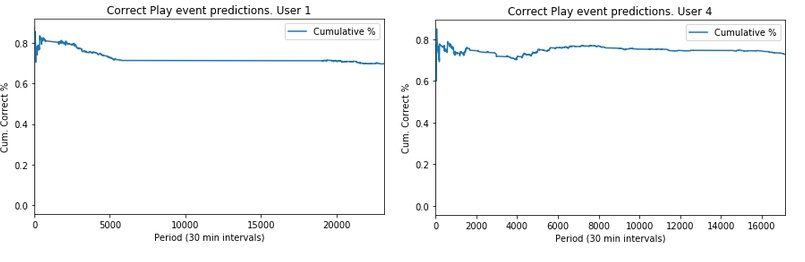
\includegraphics[width=7cm, keepaspectratio,]{fig008a.jpg}
	\caption{}
	\label{fig:fig8a}
\end{figure} 

\begin{figure}[h!]
	\centering
	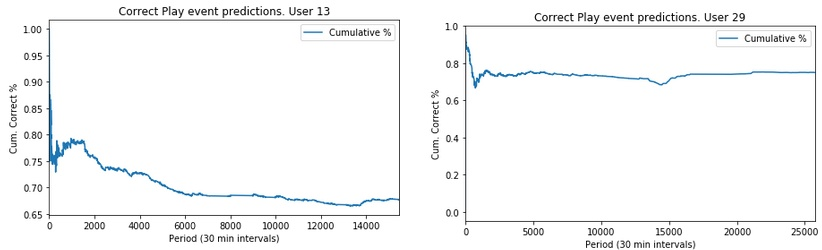
\includegraphics[width=7cm, keepaspectratio,]{fig008b.jpg}
	\caption{}
	\label{fig:fig8b}
\end{figure} 

\begin{figure}[h!]
	\centering
	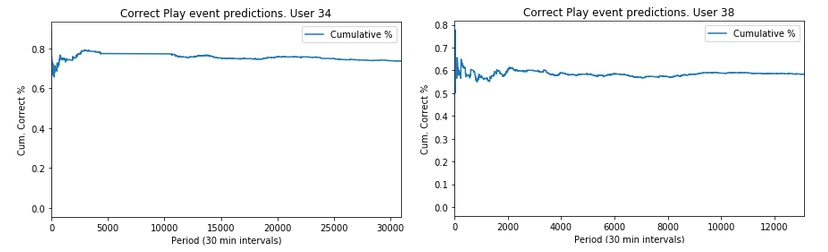
\includegraphics[width=7cm, keepaspectratio,]{fig008c.jpg}
	\caption{}
	\label{fig:fig8c}
\end{figure} 

\begin{figure}[h!]
	\centering
	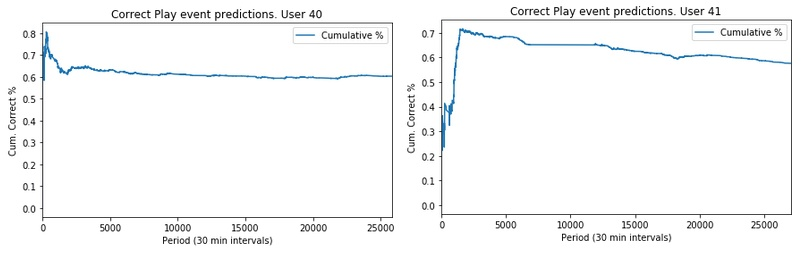
\includegraphics[width=7cm, keepaspectratio,]{fig008d.jpg}
	\caption{}
	\label{fig:fig8d}
\end{figure} 

\begin{figure}[h!]
	\centering
	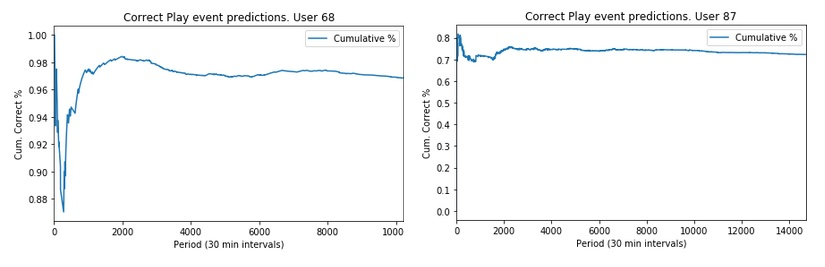
\includegraphics[width=7cm, keepaspectratio,]{fig008e.jpg}
	\caption{}
	\label{fig:fig8e}
\end{figure} 

\section{Beta-Binomial model}

\section{Logistic Regression}

\section{RNN}

